\section{Дифракция Френеля на прямолинейном краю плоского экрана и щели. Зоны Шустера, спираль Корню.}

Рассмотрим дифракцию на прямоугольной щели. Ограничимся рассмотрением плоских волн. Внимание на рисунок.

\begin{figure}[H]
	\centering
	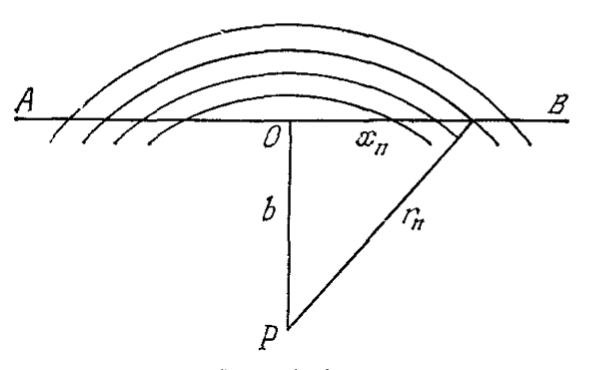
\includegraphics{31_1}
	\caption{Иллюстрация для зон Шустера}
\end{figure}

Проведем цилиндрические коаксиальные поверхности, ось которых проходит через точку $P$ перпендикулярно к плоскости рисунка, радиусы которых равны $b$, $b + \lambda/2$, $b + \lambda$ и т.д. Тогда волновой фронт разобьется на прямоугольные зоны, которые называются \textbf{зонами Шустера}. Центральную зону условимся считать сразу за две (одна слева от $O$, другая справа от $O$). В таком случае:

\begin{equation*}
	r_n^2 = b^2 + x_n^2, \quad r_{n-1}^2 = b^2 + x_{n-1}^2 \qrq r_n^2 - r_{n-1}^2 = x_n^2 - x_{n-1}^2
\end{equation*}

Приближенно мы получим:

\begin{equation*}
	r_n^2 - r_{n-1}^2 = (r_n - r_{n-1})(r_n + r_{n-1}) = 2 b (\lambda / 2) = b \lambda
\end{equation*}

Отсюда получаем рекуррентное соотношение:

\begin{equation*}
	x_n^2 - x_{n-1}^2 = b \lambda
\end{equation*}

С учетом того, что $x_0$ = 0, мы можем получить все $x_n$:

\begin{equation*}
	x_1 = \sqrt{b \lambda}, \quad x_2 = \sqrt{2 b \lambda}, \quad ..., \quad x_n = \sqrt{n b \lambda}
\end{equation*}

В таком случае ширины последовательных зон Шустера:

\begin{equation*}
	\sqrt{b \lambda}, \quad (\sqrt{2} - 1) \sqrt{b \lambda}, \quad (\sqrt{3} - \sqrt{2})\sqrt{b \lambda}
\end{equation*}

Согласно принципу Гюйгенса-Френеля волновое поле в точке $P$ представляется интегралом:

\begin{equation*}
	E_p = \int \frac{1}{r r'} e^{i \Phi(R)} d F
\end{equation*}

Заметная интенсивность наблюдается лишь при малых углах дифракции, поэтому изменениями $r r'$ можно пренебречь. Если рассматривать относительное распределение интенсивности, можно положить $r r' = 1$. В плоскости волнового фронта мы можем положить $\Phi = \omega t - k r$ (здесь мы проведем переобозначение: $r'$ из старой формулы теперь становится $r$).

Примем фазовый фронт за плоскость $XY$, начало координат положим в точке $O$. Тогда $r^2 = b^2 + (x^2 + y^2)$. Тогда $r - b = (x^2 + y^2) / (2 b) + ...$. Члены высших порядков можно отбросить (даже если вклад порядка $\pi$), т.к. они, как будет потом видно из формы полученной нами спирали, будут производить лишь незначительные смещения дифракционных максимумов и минимумов. Кроме того, высшие дифракционные максимумы и минимумы следуют друг за другом так часто, что для их реального осуществления требуются источники высокой степени монохроматичности. В противном случае они сольются в равномерный освещенный фон. Отбросим все фазовые множители, не влияющие на относительное распределение интенсивности светового поля. Тогда поле в точке $P$ оказывается равным:

\begin{equation*}
	E_p = \int \int e ^{- i k (x^2 + y^2) / (2 b)} dx dy
\end{equation*}

Пусть по оси $Y$ поле простирается довольно далеко. Тогда по $y$ можно интегрировать в пределах $-\infty, \infty$. От этого появится некоторый постоянный член, который нам не особо интересен. Интегрирование по оси $x$ произведем от 0, а верхний предел будем считать переменным ($x$). Вместо $x$ тогда введем новую переменную $s$ такую, что:

\begin{equation*}
	\frac{k x^2}{b} = \pi s^2
\end{equation*}

В таком случае получатся интегралы:

\begin{align*}
	E_p &= \int \limits_0^s e^{- i \pi s^2 / 2} d s \\
	E_p^* &= \int \limits_0^s e^{i \pi s^2 / 2} d s 
\end{align*}

Для изображения колебаний можно пользоваться любым из выражения. Для построения спирали будем пользоваться вторым выражением (в комплексной форме). В прямоугольных координатах мы в таком случае получим:

\begin{align*}
	X(s) = \int\limits_0^s \cos\left(\frac{\pi s^2}{2}\right) d s \\
	Y(s) = \int\limits_0^s \sin\left(\frac{\pi s^2}{2}\right) d s
\end{align*}

Данные интегралы называются \textbf{интегралами Френеля}. Из них видно, что получаемая кривая должна быть симметрична относительно начала координат.

Чтобы найти фокусы спирали, положим $s \rightarrow \infty$. Тогда окажется:

\begin{equation*}
	X_F = Y_F = \frac{1}{2}, \quad X_{F'} = Y_{F'} = -\frac{1}{2}
\end{equation*}

Для того, чтобы пользоваться спиралью, необходимо уметь находить $s$. Зная ширину первой зоны Шустера $\sqrt{\lambda b}$ мы далее получаем, что:

\begin{equation*}
	s = x \sqrt{\frac{2}{\lambda b}}
\end{equation*}

Для полноты картины необходимо получить графическую интерпретацию $s$. Из уравнения спирали в комплексной форме получаем для дифференциала дуги спирали:

\begin{equation*}
	\left|e^{i \pi s^2 / 2} d s\right| = |ds|
\end{equation*}

Отсюда следует, что параметр $s$ определяет длину дуги спирали, отсчитываемую от начала координат $O$.

\subsection{Дифракционная картина от прямолинейного края экрана}

Где бы ни находилась точка $P$, для нее всегда оказывается открытым первый край волнового фронта. На спирали колебание представляется вектором $\overrightarrow{M_n F}$. Если мы теперь будем двигать точку $M_n$ по спирали Корню, то мы получим распределение амплитуд и интенсивностей колебаний света по экрану. Спираль Корню представлена на рисунке ниже.

\begin{figure}[H]
	\centering
	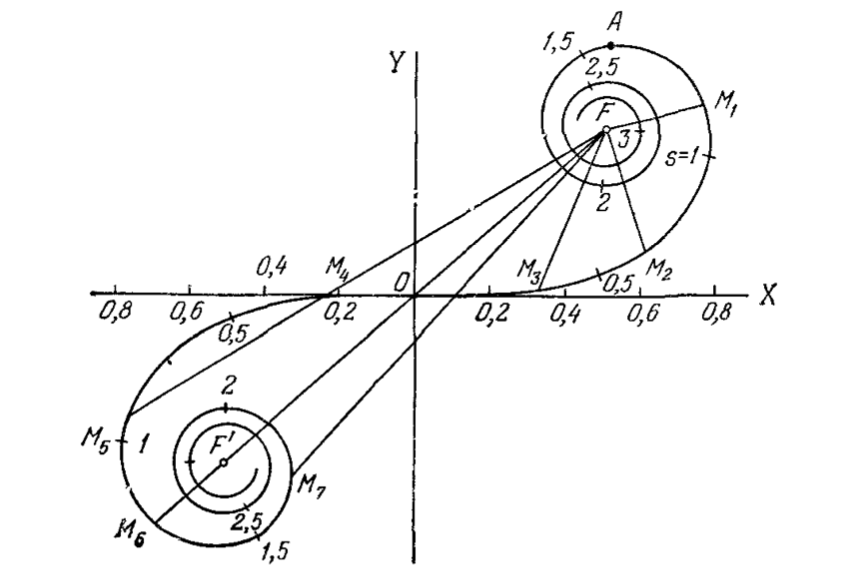
\includegraphics{31_2}
	\caption{Спираль Корню для дифракции на прямоугольном краю экрана.}
\end{figure}

Положим $a_0 = |F F'|$, $I_0 = a_0^2$ Когда точка наблюдения находится на границе геометрический тени, ей соответствует колебание, которое представимо вектором $\longrightarrow{OF} = 1/2 \longrightarrow{F'F}$. Этому соответствует амплитуда $1/2 a_0$ и, соответственно, интенсивность $1/4 I_0$. При перемещении точки в освещенную область, точка $M_n$ будет смещаться дальше по спирали и мы получим следующий график:

\begin{figure}[H]
	\centering
	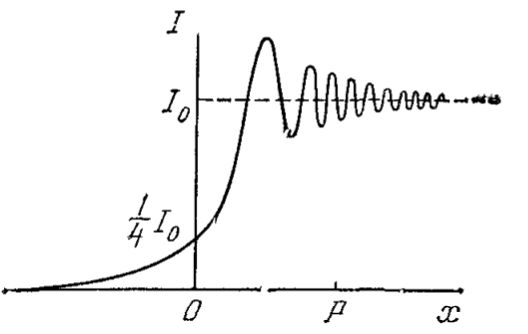
\includegraphics{31_3}
	\caption{Зависимость интенсивность от положения точки наблюдения при дифракции на прямолинейном краю экрана.}
\end{figure}





